\documentclass[12pt]{article}
\usepackage{hhline}
\usepackage{graphicx}
\graphicspath{{pictures/}}
\DeclareGraphicsExtensions{.png}
\usepackage{multirow}
\usepackage{amsmath}
\usepackage{mathtext}
\usepackage[T2A]{fontenc}
\usepackage[utf8]{inputenc}
\usepackage{pscyr} 
\usepackage[left=2cm,right=2cm, top=1.5cm,bottom=1cm,bindingoffset=0cm]{geometry}

\begin{document}
\pagestyle{empty}
\begin{center}
\large{\textbf{Университет ИТМО}}
\end{center}
\rule{500pt}{1pt}
\par\bigskip\par\bigskip\par\bigskip\par\bigskip\par\bigskip\par\bigskip\par\bigskip\par\bigskip
\begin{center}
\Large
\textbf{Отчёт по лабораторной работе №2}

\textbf{\textit{«Изучение центрального соударения тел.}}

\textbf{\textit{Проверка второго закона Ньютона»}}
\end{center}
\par\bigskip\par\bigskip\par\bigskip\par\bigskip\par\bigskip\par\bigskip\par\bigskip\par\bigskip\par\bigskip\par\bigskip\par\bigskip\par\bigskip\par\bigskip\par\bigskip      
\begin{flushright}
\large
Выполнил: Федюкович С. А.
\par\bigskip
Факультет: МТУ “Академия ЛИМТУ”
\par\bigskip
Группа: S3100                       
\par\bigskip\par\bigskip\par\bigskip

\rule{150pt}{0.5pt}
\par\bigskip\par\bigskip\par\bigskip\par\bigskip                                                            
 Проверил: Пшеничников В. Е. 
\par\bigskip \par\bigskip

\rule{150pt}{0.5pt}
\end{flushright}
\par\bigskip\par\bigskip\par\bigskip\par\bigskip\par\bigskip\par\bigskip\par\bigskip\par\bigskip\par\bigskip\par\bigskip     
\begin{center}
\large
Санкт-Петербург
\par\bigskip
2018
\end{center}
\newpage

\section*{Цель работы}
\begin{enumerate}
\itemЭкспериментальная проверка законов упругого и неупругого центрального соударения для системы двух тележек, движущихся с малым трением.
\itemИсследование зависимости ускорения тележки от приложенной силы и массы тележки.
\end{enumerate}

\section*{Теоретические основы лабораторной работы}
\subsection*{Часть 1}
Рассмотрим абсолютно упругое центральное соударение двух тел массами $m_{1}$  и $m_{2}$  , при таком соударении в замкнутой системе двух тел выполняются законы сохранения импульса и энергии. Пусть до соударения движется только первое тело, тогда уравнения законов имеют вид:
\begin{equation}
\Large
 \begin{cases}
   m_{1}\vec{v}_{10}=m_{1}\vec{v}_{1}+m_{2}\vec{v}_{2}\\
  \frac{ m_{1}v_{10}^2}{2}=\frac{ m_{1}v_{1}^2}{2}+\frac{ m_{2}v_{2}^2}{2}
 \end{cases},
\end{equation}
где $\vec{v}_{10}$ --- скорость первого тела до удара, $\vec{v}_{1}$и $\vec{v}_{2}$ --- соответственно, скорости первого и второго тел после удара. Считая скорость $\vec{v}_{10}$ известной, найдем скорости обоих тел после удара. Пусть условия соударения таковы, что после удара оба тела продолжают двигаться параллельно той прямой, по которой двигалось первое тело до удара. 
\begin{center}
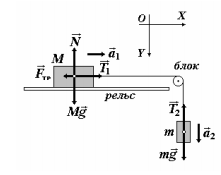
\includegraphics{part2}
\end{center}

Введем координатную ось $OX$, сонаправленную с вектором $\vec{v}_{10}$. Для проекций скоростей $v_{1}$, $v_{2}$ из уравнений $(1)$ получим систему двух уравнений:\begin{equation}
\Large
 \begin{cases}
   m_{1}v_{10}=m_{1}v_{1x}+m_{2}v_{2x}\\
  \frac{ m_{1}v_{10}^2}{2}=\frac{ m_{1}v_{1x}^2}{2}+\frac{ m_{2}v_{2x}^2}{2}
 \end{cases}
\end{equation}	
Умножим все слагаемые второго уравнения на два, и перенесем налево в обоих уравнениях слагаемые, характеризующие импульс и энергию первого тела:
\begin{equation}
\Large
 \begin{cases}
   m_{1}(v_{10}-v_{1x})=m_{2}v_{2x}\\
   m_{1}(v_{10}^2-v_{1x}^2)= m_{2}v_{2x}^2
 \end{cases}
\end{equation}
После удара скорость первого тела должна измениться. Поэтому содержимое скобок в левых частях уравнений $(3)$ отлично от нуля, и для упрощения системы можно поделить левые и правые части нижнего уравнения на соответствующие части верхнего уравнения. Результат деления сделаем вторым уравнением системы:
\begin{equation}
\Large
 \begin{cases}
   m_{1}(v_{10}-v_{1x})=m_{2}v_{2x}\\
   v_{10}-v_{1x}= v_{2x}
 \end{cases}
\end{equation}
Отсюда нетрудно найти окончательные выражения для скоростей:
\begin{equation}
\Large
 \begin{cases}
   v_{1x}=\frac{(m_{1}- m_{2})v_{10}}{m_{1}+m_{2}}\\
   v_{2x}=\frac{2m_{1}v_{10}}{m_{1}+m_{1}}
 \end{cases}
\end{equation}
Из первого уравнения $(5)$ следует, что в зависимости от соотношения масс первое тело после соударения может: 

а) продолжить движение вперед ($m_{1}>m_{2}$,$v_{1x}>0$);

б) остановится ($m_{1}=m_{2}$,$v_{1x}=0$);

в) поменять направление движения на противоположное ($m_{1}<m_{2}$,$v_{1x}<0$).

При абсолютно неупругом соударении рассмотренных выше тел, оба тела после удара двигаются как одно целое с суммарной массой. В этом случае законы сохранения импульса и энергии принимают вид:
\begin{equation}
\Large
 \begin{cases}
   m_{1}\vec{v}_{10}=(m_{1}+m_{2})\vec{v}\\
  \frac{ m_{1}v_{10}^2}{2}=\frac{(m_{1}+m_{2})\vec{v}}{2} + W_{пот}
 \end{cases}
\end{equation}
Здесь $\vec{v}$– скорость тел после соударения, $W_{пот}$ – потери механической энергии при соударении.

В первом уравнении $(6)$ равенство векторов означает равенство их модулей, и для модуля скорости тел после соударения из этого уравнения находим:
\begin{equation}
\Large
  v=\frac{m_{1} v_{10}}{m_{1}+m_{2}}
\end{equation}
Подставив во второе уравнение системы $(6)$ вместо скорости v правую часть уравнения $(7)$, получим следующее выражение для потерь механической энергии при соударении:
\begin{equation}
\Large
 W_{пот}=\frac{m_{1}m_{2}v_{10}^2}{2(m_{1}+m_{2})}
\end{equation}
Относительные потери механической энергии при неупругом соударении вычисляются по формуле:
\begin{equation}
\Large
\frac{W_{пот}}{ \frac{ m_{1}v_{10}^2}{2}}=\frac{m_{2}}{m_{1}+m_{2}}
\end{equation}
В качестве соударяющихся тел в лабораторной работе выступают две тележки, скользящие с малым трением по горизонтальному рельсу.
\subsection*{Часть 2}


Рассмотрим систему, состоящую из тележки $M$ и гирьки $m$, соединенных невесомой нерастяжимой нитью. Тележка с небольшим трением скользит по горизонтальному рельсу. 
Масса блока, через который перекинута нить, пренебрежимо мала.
\begin{center}
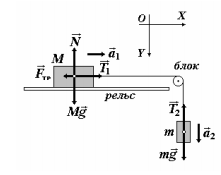
\includegraphics{part2}
\end{center}
Уравнения второго закона Ньютона для тележки и гирьки, соответственно, имеют вид:
\begin{equation}
\Large
M\vec{a}_{1}=M\vec{g}+\vec{N}+\vec{T}_{1}+\vec{F}_{тр}
\end{equation}
\begin{equation}
\Large
m\vec{a}_{2}=m\vec{g}+\vec{T}_{2} 
\end{equation}
Здесь $\vec{a}_{1}$,$\vec{a}_{2}$ --- ускорения тележки и гирьки; $\vec{N}$ --- сила реакции опоры, $\vec{T}_{1}$, $\vec{T}_{2}$ --- силы натяжения нити, $\vec{F}_{тр}$ --- сила трения. Из-за нерастяжимости нити модули обоих ускорений равны друг другу, обозначим их одной буквой: $a_{1}=a_{2}=a$. Из-за невесомости нити и блока можно также 
принять: $T_{1}=T_{2}=T$.
Для проекций векторов на координатные оси из уравнения $(10)$ получаем:
\begin{equation}
\Large
 \begin{cases}
  OY: N = Mg \\
OX: Ma=T-F_{тр}
 \end{cases};
\end{equation}
из уравнения $(11)$:
\begin{equation}
\Large
 \begin{cases}
  OY: ma = mg - T
 \end{cases}.
\end{equation}
\newpage
\section*{Экспериментальные данные}
\subsection*{Упражнение 1}
\begin{center}
Таблица 1.1. Зависимость скорости тел при абсолютно упругом соударении без утяжелителя 
\begin{table}[h!]
\begin{center}
\begin{tabular}{|c|c|c|c|c|c|}
\hline
 № & Тело 1 & Тело 2 & $v_{10x}$, м/c & $v_{1x}$, м/c & $v_{2x}$, м/c \\
\hline
 1 &\multirow{5}{60pt}{Тележка 1 + втулка с рогаткой}    & \multirow{5}{60pt}{Тележка 2 + втулка с рогаткой} & 0,53&	0,06	&0,43 \\
\hhline{-~~---}

 2 &    &  & 0,54&	0,06	&0,43 \\
\hhline{-~~---}
 3 &   &  & 0,57&	0,07&	0,43 \\
\hhline{-~~---}
 4 &  &  &0,55	&0,05&	0,47 \\
\hhline{-~~---}
 5 &    &  & 0,55&	0,05&	0,45 \\
\hline
\end{tabular}

Приборные погрешности:$\Delta v_{10}=\Delta v_{1}=\Delta v_{2} = 0,01$ м/c. 
\end{center}
\end{table} 

Таблица 1.2. Зависимость скоростей тел при абсолютно упругом столкновении с утяжелителем
\begin{table}[h!]
\begin{center}
\begin{tabular}{|c|c|c|c|c|c|}
\hline
 № & Тело 1 & Тело 2 & $v_{10x}$, м/c & $v_{1x}$, м/c & $v_{2x}$, м/c \\
\hline
 1 &\multirow{5}{70pt}{Тележка 1 + втулка с рогаткой}    & \multirow{5}{70pt}{Тележка 2 + втулка с рогаткой + утяжелитель} & 0,55&	-0,08&	0,28 \\
\hhline{-~~---}

 2 &    &  & 0,54&	-0,10&	0,26 \\
\hhline{-~~---}
 3 &   &  &0,55	&-0,09	&0,26 \\
\hhline{-~~---}
 4 &  &  &0,53&	-0,09	&0,28 \\
\hhline{-~~---}
 5 &    &  & 0,52&	-0,08	&0,25 \\
\hline
\end{tabular}
\end{center}
\end{table}

Таблица 2.1. Зависимость скоростей тел при абсолютно неупругом столкновении без утяжелителя
\begin{table}[h!]
\begin{center}
\begin{tabular}{|c|c|c|c|c|}
\hline
 № & Тело 1 & Тело 2 & $v_{10x}$, м/c & $v$, м/c \\
\hline
 1 &\multirow{5}{70pt}{Тележка 1 + втулка с липучкой}    & \multirow{5}{70pt}{Тележка 2 + втулка с липучкой} & 0,56&	0,23 \\
\hhline{-~~--}

 2 &    &  & 	0,54&	0,21 \\
\hhline{-~~--}
 3 &   &  &0,47&	0,19 \\
\hhline{-~~--}
 4 &  &  &	0,48&	0,20 \\
\hhline{-~~--}
 5 &    &  &	0,49&	0,20 \\
\hline
\end{tabular}
\end{center}
\end{table}

Таблица 2.2. Зависимость скоростей тел при абсолютно неупругом столкновении с утяжелителем
\begin{table}[h!]
\begin{center}
\begin{tabular}{|c|c|c|c|c|}
\hline
 № & Тело 1 & Тело 2 & $v_{10x}$, м/c & $v$, м/c \\
\hline
 1 &\multirow{5}{70pt}{Тележка 1 + втулка с липучкой}    & \multirow{5}{70pt}{Тележка 2 + втулка с липучкой + утяжелитель} & 0,56&	0,11 \\
\hhline{-~~--}

 2 &    &  & 	0,56	&0,13 \\
\hhline{-~~--}
 3 &   &  &0,53	&0,15 \\
\hhline{-~~--}
 4 &  &  &	0,49&	0,07 \\
\hhline{-~~--}
 5 &    &  &	0,50&	0,15 \\
\hline
\end{tabular}
\end{center}
\end{table}                        
\end{center}
\newpage
\subsection*{Упражнение 2}
\begin{center}
$x_{1} = 0,150$ м; $x_{2} = 0,800$ м. Погрешности координат примем $\Delta x_{1} = \Delta x_{2}  = 5$ мм

Таблица 3.1. Зависимость времени от количества шайб без утяжелителя
\begin{table}[h!]
\begin{center}
\begin{tabular}{|c|c|c|c|}
\hline
 № & Состав подвески & $t_{1}$, c & $t_{2}$, c \\
\hline
 1 &    крючок &	0,29	 &0,69 \\
\hline

 2 & крючок + 1 шайба &	0,36	 &0,84 \\
\hline
 3 &  крючок + 2 шайба &	0,41 &	0,96 \\
\hline
 4 &крючок + 3 шайба &	0,46	 &1,07 \\
\hline

\end{tabular}

Приборные погрешности:$\Delta t_{1}=\Delta t_{2} = 0,05$ c. 
\end{center}
\end{table}

Таблица 3.2. Зависимость времени от количества шайб с утяжелителем
\begin{table}[h!]
\begin{center}
\begin{tabular}{|c|c|c|c|}
\hline
 № & Состав подвески & $t_{1}$, c & $t_{2}$, c \\
\hline
 1 &    крючок + утяжелитель&	0,19&	0,48\\
\hline

 2 & крючок + утяжелитель + 1 шайба&	0,24&	0,59 \\
\hline
 3 & крючок + утяжелитель + 2 шайбы&	0,29&	0,68 \\
\hline
 4 &крючок + утяжелитель + 3 шайбы	&0,32&	0,76 \\
\hline
\end{tabular}
\end{center}
\end{table}             
\end{center}

\section*{Обработка результатов измерений}
\subsection*{Упражнение 1}
\begin{enumerate}
\item Оценим относительные потери импульса и кинетической энергии за счет
трения по формулам:
\begin{equation}
\Large
\partial^{(тр)}_{p} = \frac{\Delta p}{p} = \frac{v\rq{}}{v} - 1 ; \partial^{(тр)}_{W} = \frac{\Delta W_{к}}{W_{к}} = \frac{v\rq{}^2}{v^2} - 1 .
\end{equation}
\itemС помощью таблицы масс для таблицы 1.1 рассчитаем массы $m_{1}$, $m_{2}$
соударяющихся тел. Найденные значения занести в таблицу 4.1 . По данным
таблицы 1.1 рассчитаеи и занесем в таблицу 4.1 импульсы тел:
\begin{equation}
\Large
p_{10x}=m_{1}v_{10x},  p_{1x}=m_{1}v_{1x}, p_{2x}=m_{2}v_{2x}.
\end{equation}
\begin{table}[h!]
\begin{center}
\begin{tabular}{|c|c|c|c|c|c|c|c|}
\hline
 № & $m_{1}$, г & $m_{2}$, г  & $p_{10x}, мН\cdot с$ &$p_{1x}, мН\cdot с$ &$p_{2x}, мН\cdot с$ & $\partial_{p}$& $\partial_{W}$\\
\hline
 1 &\multirow{5}{*}{49,5}& \multirow{5}{*}{51,5}& 26,23&	2,97	&22,14&	-0,04&	-0,30\\
\hhline{-~~-----}

 2 &    &  & 	26,73	 &2,97 &22,14	 &-0,06	 &-0,39 \\
\hhline{-~~-----}
 3 &   &  &28,21 &	3,46 &	22,14 &	-0,09	 &-0,39 \\
\hhline{-~~-----}
 4 &  &  &27,22	 &2,47 &	24,20	 &-0,02 &	-0,23 \\
\hhline{-~~-----}
 5 &    &  &27,22 &	2,47 &	23,17 &	-0,05 &	-0,29 \\
\hline
\end{tabular}
\end{center}
\end{table}                        
\item Вычислим для каждой строки 4.1 относительные изменения импульса и
кинетической энергии системы при соударении по формулам:
\begin{equation}
\Large
\partial_{p} = \Delta P_{x} / p_{10x}=\frac{p_{1x} + p_{2x}}{p_{10x}} - 1 
\end{equation}
\begin{equation}
\Large
\partial_{p} = \Delta W_{к} / W_{к0}=\frac{m_{1}v^2_{1x}+m_{2}v^2_{2x}}{m_{1}v^2_{10x}} - 1
\end{equation}
Занесем результаты в таблицу. Рассчитаем средние значения $\overline{\partial}_{p}, \overline{\partial}_{W}$
относительных потерь импульса и энергии по двум последним колонкам
таблицы 4.1:
\begin{equation}
\large
\overline{\partial}_{p} = \frac{\sum_{i=1}^N \partial_{pi}}{N}  \approx -0,5; 
\overline{\partial}_{W} = \frac{\sum_{i=1}^N\partial_{Wi}}{N}  \approx -0,32.
\end{equation}

Здесь $i$ – номер опыта, $N$ общее число опытов. По разбросу отдельных значений
$\partial_{p},\partial_{W}$ найдем погрешности их средних значений:

\begin{equation}
\Delta \overline{\partial_{p}} = K_{S}(\alpha_{дов}, N) \sqrt{ \frac{\sum_{i=1}^N(\partial_{pi}-\overline{\partial}_{p})^2}{N(N-1)}} \approx 0,01;
\Delta \overline{\partial_{W}} = K_{S}(\alpha_{дов}, N) \sqrt{ \frac{\sum_{i=1}^N(\partial_{Wi}-\overline{\partial}_{W})^2}{N(N-1)}} \approx 0,04,
\end{equation}
где $K_{S}(\alpha_{дов}, N)$ – коэффициент Стьюдента для доверительной вероятности
$\alpha_{дов}= 0,7$ и количества измерений $N$. Сравним разности $\overline{\partial_{p}} -\partial^{(тр)}_{p},\overline{\partial_{W}} -\partial^{(тр)}_{W}$
соответствующими неопределенностями $(19)$.
\item По данным таблиц 1.2 вычислим импульсы $(15)$ и относительные
изменения импульса и энергии $(16)$, $(17)$. Результаты представим в таблицах
4.2:


По двум последним колонкам таблицы 4.2
найдём средние значения $\overline{\partial}_{p}, \overline{\partial}_{W}$ и сравним их, соответственно, с $\overline{\partial}^{(тр)}_{p}, \overline{\partial}^{(тр)}_{W}$
\item По данным из таблицы 2.1 заполнить следующую таблицу .

Здесь $m_{1}, m_{2}$ – массы соударяющихся тел;
\begin{equation}
p_{10}= m_{1}v_{10} -импульс\: системы\: до\: соударения; 
\end{equation}
\begin{equation}
p = (m_{1} m_{2})v - импульс\: системы \:после\: соударения;
\end{equation}
\begin{equation}
\partial_{p} = \Delta p/ p_{10} = (\frac{p_{1}}{p_{10}} -1)  - относительное\: изменение\: импульса;
\end{equation}

$\partial^{(э)}_{W}$ --- экспериментальное значение относительного изменения механической
энергии, вычисляемое по формуле:
\begin{equation}
\partial^{(э)}_{W} = \Delta W_{к}/ W_{к0} = \frac{(m_{1}+m_{2})v^2_{2}}{m_{1}v^2_{10}} - 1,
\end{equation}
$\partial^{(т)}_{W}$---теоретическое значение относительного изменения механической
энергии, вычисляемое по формуле $(9)$. Вычислим средние значения $\overline{\partial}_{p}$ и $\overline{\partial}^{(э)}_{W}$. Сравним
$\overline{\partial}_{p}$ и $\partial^{(тр)}_{p}$. Найдем разность между величинами $\overline{\partial}^{(э)}_{W}$ и $\partial^{(т)}_{W}$, сравнить её с величиной $\partial^{(тр)}_{W}$.
\item Выполнить вычисления пункта 5 для данных из таблицы 2.2, заполнив
таблицу 5.2:
\end{enumerate}

\end{document}